\documentclass[a4paper]{article}

\usepackage{../../../settings}


\begin{document}

Consider the following function, which decomposes the integer $x$ into prime factors. Let the number $x$ not exceed $C$. Estimate the asymptotic behavior of the running time of this function.

\SPACE

\noindent C++:

\begin{lstlisting}[style=C++]
#include <vector>

std::vector<int> primes(int x) {
    std::vector<int> result;
    int i = 2;
    while (i * i <= x) {
        while (x % i == 0) {
            result.push_back(i);
            x /= i;
        }
        ++i;
    }
    if (x != 1) {
        result.push_back(x);
    }
    return result;
}
\end{lstlisting}

\SPACE

\noindent Python:

\begin{lstlisting}[style=Python]
def primes(x):
    result = []
    i = 2
    while i * i <= x:
        while x % i == 0:
            result.append(i)
            x //= i
        i += 1
    if x != 1:
        result.append(x)
    return result
\end{lstlisting}

\SPACE

\LINE

\SPACE

\begin{itemize}
\item $O(\sqrt{C} + \log C)$
\item $O(\sqrt{C} \log C)$
\item $O(\log C)$
\item {\color{OliveGreen}{$\mathbf{O(\sqrt{C})}$}}
\item $O(C)$
\end{itemize}

\SPACE

\newpage

In the worst case, the algorithm does not go into the inner loop and iterates in the outer $\sqrt{C}$ times. In general, $x$ decreases logarithmically, reducing complexity.

\begin{center}
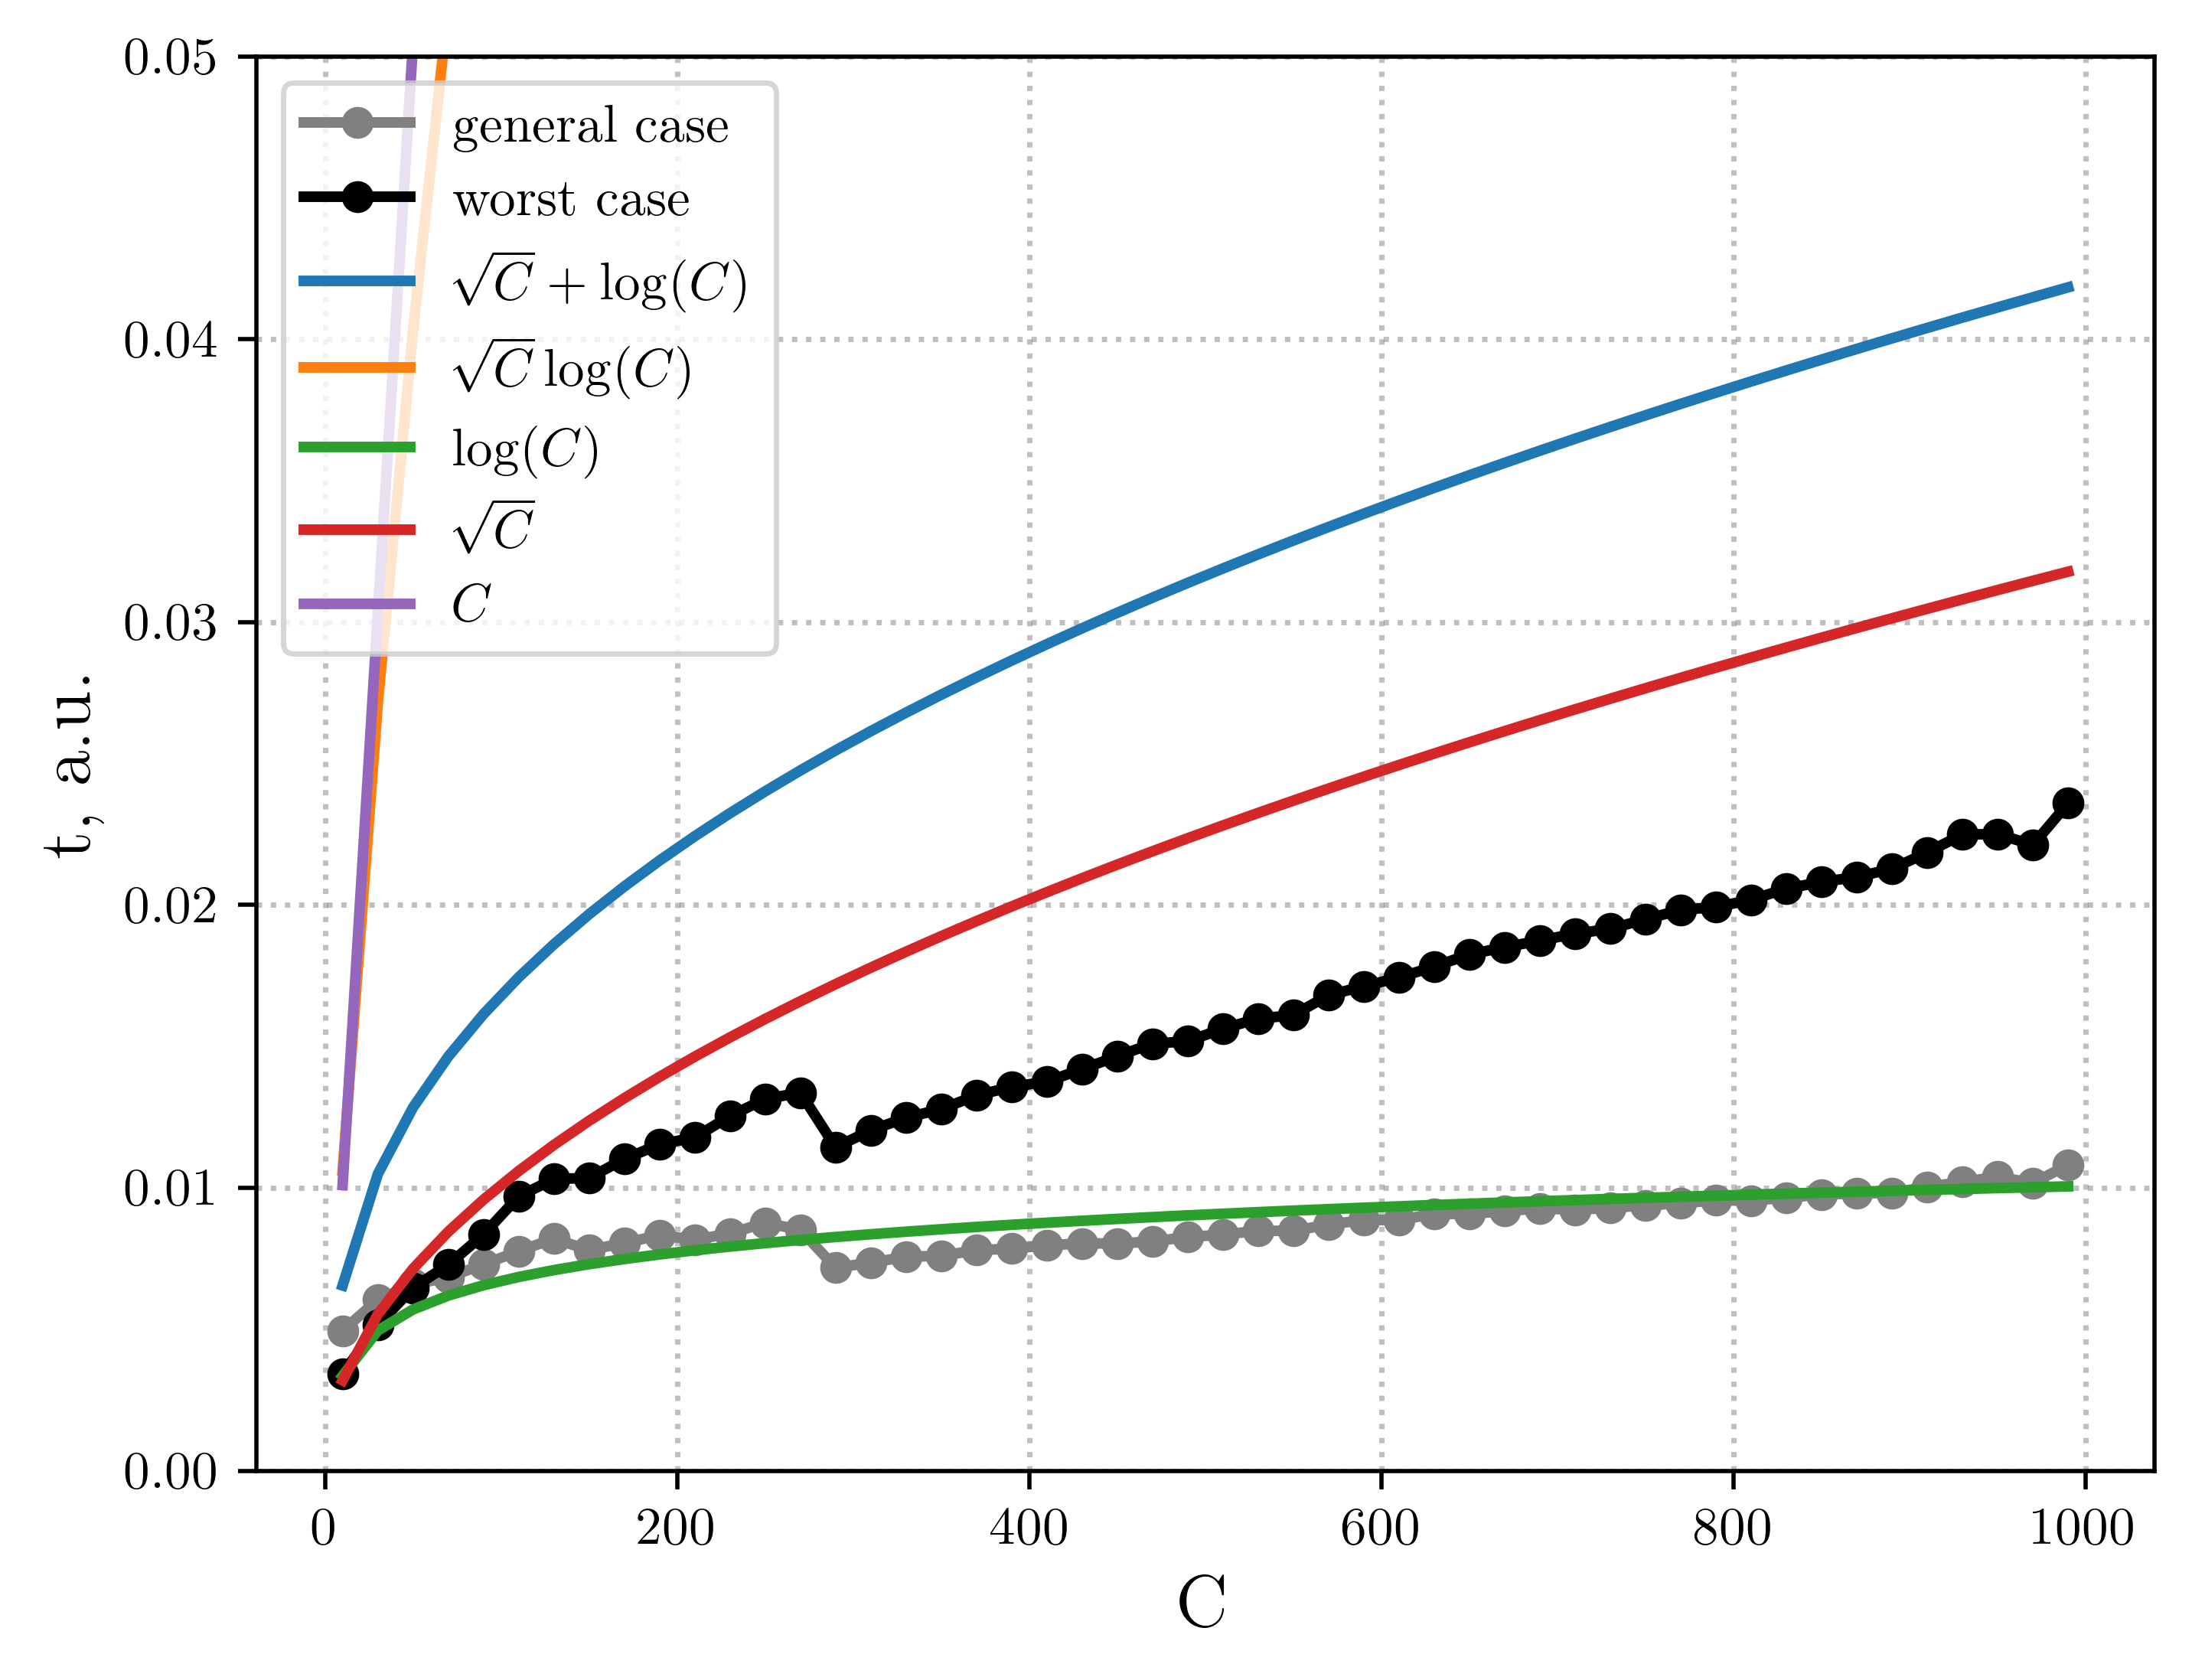
\includegraphics[width=15cm]{06.png}
\end{center}

\end{document}